\section{Pseudocode \& Algoritmes}
\subsection{Uitleg}

\begin{frame}
\frametitle{Hoe zet je een probleem om in een programma?}

\begin{itemize}
  \item<1-> Begin met het probleem te versimpelen.
  \item<2-> Denk vervolgens als een computer:
  \begin{itemize}
  	\item<3-> Niets is ``duidelijk'' of ``obvious'': 
	  \begin{itemize}
	  	\item<4-> De computer denkt niet zelf na!
	  \end{itemize}
  	\item<5-> Je moet alles letterlijk uitspellen voor de computer!
  \end{itemize}
  \item<6-> Het helpt om gebruik te maken van ``pseudocode''.
\end{itemize}

\end{frame}



\begin{frame}
\frametitle{Wat is pseudocode?}

\begin{itemize}
  \item<1-> Pseudocode ligt tussen ``echte'' code en mensentaal in.
  \begin{itemize}
  	\item<2-> ``Echte'' code heeft een strakke syntax waar je je aan moet houden.
  	\begin{itemize}
  	  \item<3-> Een kleine typefout en de computer begrijpt je niet!
  	\end{itemize}
  	\item<4-> Pseudocode heeft niet zo'n strakke syntax,\\maar het is ``in eigen woorden''
  \end{itemize}
  \item<5-> Pseudocode heeft echter wel de \textbf{structuur} van een stukje code
\end{itemize}

\end{frame}




\begin{frame}
\frametitle{Wat is pseudocode?}
\framesubtitle{Voorbeeld}

Stel dat we een programma willen schrijven die ons vertelt of we vandaag een paraplu nodig hebben.
\visible<2>{In pseudocode:}


\visible<2->{
\begin{minipage}{0.7\textwidth}%
	\begin{algorithm}[H]
	\caption{Pseudocode ``paraplu nodig?''}
	\begin{algorithmic}[1]
	\Function{ParapluNodig}{regenkans}
	   \If{regenkans = hoog}
	     \State Paraplu nodig
	   \ElsIf{regenkans = laag}
	     \State Geen paraplu nodig
	   \Else
	     \State Paraplu optioneel. \Comment{Je smelt niet!}
	   \EndIf
	\EndFunction
	\end{algorithmic}
	\end{algorithm}
\end{minipage}%
\visible<3->{
\begin{minipage}{0.27\textwidth}%
	\begin{ticalc}
		PROGRAM\:PARAPLU\\%
		\:Prompt\,R\\%
		\:If\,R>40\\%
		\:Then\\%
		\:Disp\,\qt PARAPLU\,NODIG\qt\\%
		\:Else\:If\,R<10\\%
		\:Then\\%
		\:Disp\,\qt PARAPLU\,ONNODIG\qt\\%
		\:Else\\%
		\:Disp\,\qt PARAPLU\,OPTIONEEL\qt\\%
		\:End
		\:End
	\end{ticalc}
\end{minipage}%	
}
}


\addtocounter{algorithm}{-1} % Prevents the algorithm number to increase every frame
\end{frame}
\addtocounter{algorithm}{1} % Make sure the number increases for a new algorithm on a different slide


\begin{frame}
\frametitle{Wat is het nut van pseudocode?}

Wanneer een programma zeer ingewikkeld wordt, kun je soms honderden regels code samenvatten in slechts 1 zin pseudocode.
Bijv. ``bereken het elektrisch veld'', zoals in de figuur hieronder.

\visible<2->{
\begin{figure}[h]
\centering
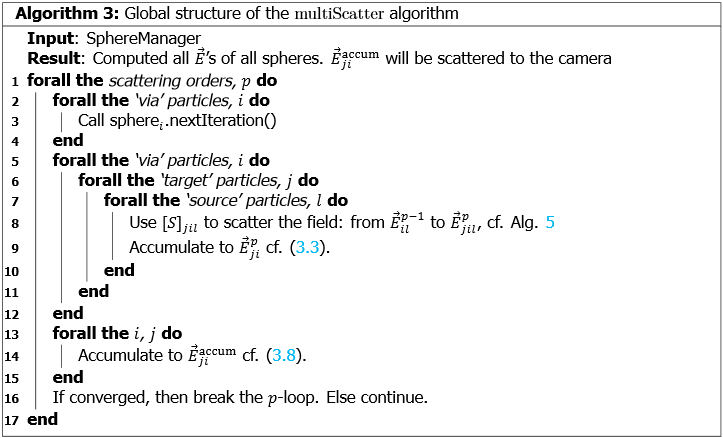
\includegraphics[height=0.6\textheight]{../figures/AlgorithmMScThesis.png}
\end{figure}
\tiny{Deze figuur komt uit mijn master afstudeerproject: http://www.kevinvanas.nl/TUDelft/MSc/Report.pdf}
}

\end{frame}


\begin{frame}
\frametitle{Wat is een algoritme?}

\begin{itemize}
  \item<1-> Op voorgaande slides kwam het woord ``\textbf{Algorithm}'' voor (NL: Algoritme). Wat is dat?
  \item<2-> Een algorithme is ``een stukje code''.
  \item<3-> Dat ``stukje code'' heeft als doel om iets specifieks uit te rekenen.
  \begin{itemize}
    \item<4-> Bijvoorbeeld het uitrekenen van het zesde priemgetal\only<5->{ ($=13$)}.
  \end{itemize}
  \item<5-> Dus overal waar ``Algorithm'' staat, kun je simpelweg denken ``\emph{een stukje computercode om iets uit te rekenen}''.
\end{itemize}

\end{frame}


\subsection{Zelf Oefenen}

\begin{frame}
\frametitle{Oefening: Wat doet deze pseudocode?}

\begin{algorithm}[H]
\caption{Pseudocode ``WhatDoIDo?''}
\begin{algorithmic}[1]
% ABC formule
\Function{WhatDoIDo}{$a$,$b$,$c$}
	\State $D=\sqrt{b^2-4ac}$
	\If{$D>0$}
		\State Er zijn twee oplossingen
		\State $x = (-b\pm D) / 2a$
	\ElsIf{$D=0$}
		\State Er is exact \'e\'en oplossing
		\State $x = -b / 2a$
	\Else \Comment{$D<0$}
		\State Er zijn geen re\"ele oplossingen!
	\EndIf
\EndFunction
\end{algorithmic}
\end{algorithm}

\end{frame}




\begin{frame}
\frametitle{Oefening: Wat doet deze pseudocode?}

\begin{algorithm}[H]
\caption{Pseudocode ``WhatDoIDo2?''}
\begin{algorithmic}[1]
% Risk dobbelstenen
\Function{WhatDoIDo2}{$N_{att}$}
	\State Maak $N_{att}$ random getallen tussen $1$ en $6$
	\State Vraag of $N_{def}$ $1$ of $2$ is
	\State Maak $N_{def}$ random getallen tussen $1$ en $6$
	\State Sorteer beide setten van hoog naar laag
	\If{Getal 1 van set 1 > Getal 1 van set 2}  $p_1=p_1+1$
	\Else \hspace{0.4cm} $p_2=p_2+1$
	\EndIf
	\If{Getal 2 van set 1 > Getal 2 van set 2}  $p_1=p_1+1$
	\Else \hspace{0.4cm} $p_2=p_2+1$
	\EndIf
	\State Display de scores: $p_1$ en $p_2$
\EndFunction
\end{algorithmic}
\end{algorithm}


\end{frame}




\begin{frame}
\frametitle{Oefening: Wat doet deze pseudocode?}

\begin{algorithm}[H]
\caption{Pseudocode ``WhatDoIDo3?''}
\begin{algorithmic}[1]
% Spraakherkenning
\Function{WhatDoIDo3}{geluid $g$}\Comment{Niet voor GR geschikt}
\State Knip $g$ op in losse klanken, $k$.
\State Laad een database in.
\State Verwijder de stiltes uit $k$.
\State Correleer $k$ met alle items in de database.
\State Bereken een score voor alle klanken en vind daarmee de meest waarschijnlijke letter.
\State Maak een lijst voor alle mogelijke woorden die $g$ kan zijn.
\State Vergelijk de lijst met een woordenboek en kies het meest waarschijnlijke woord.
\EndFunction
\end{algorithmic}
\end{algorithm}


\end{frame}



\begin{frame}\label{frame:pseudo_exercises}
\frametitle{Nu jullie: Maak je eigen pseudocode!}

\begin{enumerate} 
  \item Bepaal of iemand genoeg geld, $g$, op zijn rekening heeft staan, indien hij een product voor $x$ euro wil kopen
  	en $r$ euro in het rood mag staan.
  \item Gegeven de huidige datum, $(y_t, m_t, d_t)$, en iemand's geboortedatum, $(y_g, m_g, d_g)$, bepaal zijn/haar leeftijd.
  \item Uit een set van 5 kaarten, bepaal wat de pokerset is.
  \begin{itemize}
    \item Bijvoorbeeld: ``pair of $5$'s, $K$ high'' or ``straight, $9$ high''
  \end{itemize}
  \item Er zijn vier spelers die elk punten hebben. Bepaal de winnaar, i.e. degene met de meeste punten.
  \item Bereken de `rest' van $y/x$.
  \begin{itemize}
    \item Bijvoorbeeld: $5/2 = 2$ `rest' $1$
    \item Tip: Kijk naar \tiMATH\inlineticalc{NUM}\inlineticalc{int(} of \tiMATH\inlineticalc{NUM}\inlineticalc{fPart(}
  \end{itemize}
\end{enumerate}

\end{frame}






\begin{frame}
\frametitle{Zet pseudocode om in een \tifonttxt{Prgm}!}

Implementeer deze twee opdrachten van de vorige slide op je rekenmachine:

\begin{enumerate} 
  \item Bepaal of iemand genoeg geld, $g$, op zijn rekening heeft staan, indien hij een product voor $x$ euro wil kopen
  	en $r$ euro in het rood mag staan.
  \item Gegeven de huidige datum, $(y_t, m_t, d_t)$, en iemand's geboortedatum, $(y_g, m_g, d_g)$, bepaal zijn/haar leeftijd.
  \begin{itemize}
    \item Tip: Het is handig om voor jezelf duidelijk 6 variabelen te kiezen \emph{\'en} op te schrijven wat alles betekent.
    	Immers, je kunt slechts \'e\'en letter gebruiken per variabele! Duidelijkheid is zeer belangrijk:
    	Als je het overzicht verliest, dan weet je zeker dat je je \tifonttxt{Prgm} niet kunt schrijven.
  \end{itemize}
\end{enumerate}



\end{frame}





